\documentclass[12pt,a4paper,article,english,firamath]{nsi}
\pagestyle{empty}
\setfontfamily{\brettley}{Cursive standard}[Scale=1.5]
\begin{document}
\titre{Find your figure}
\classe{Euro 1\ere}
\maketitle

\subsection*{Description 7}
{\brettley 

Draw a segment and divide it into two equal parts. Draw a circle passing through one endpoint and the midpoint, with its
center on the segment. Do the same with the other half of the segment. Then, draw a line segment perpendicular to the
first segment, passing through is midpoint, with the same length. Finally, join the endpoints of the two segments with
two pairs of parallel lines.}\\[1em]

\begin{tikzpicture}
    \draw[lightgray](0,0)--(\linewidth,0);
\end{tikzpicture}


\subsection*{Figure 7}
\begin{center}
    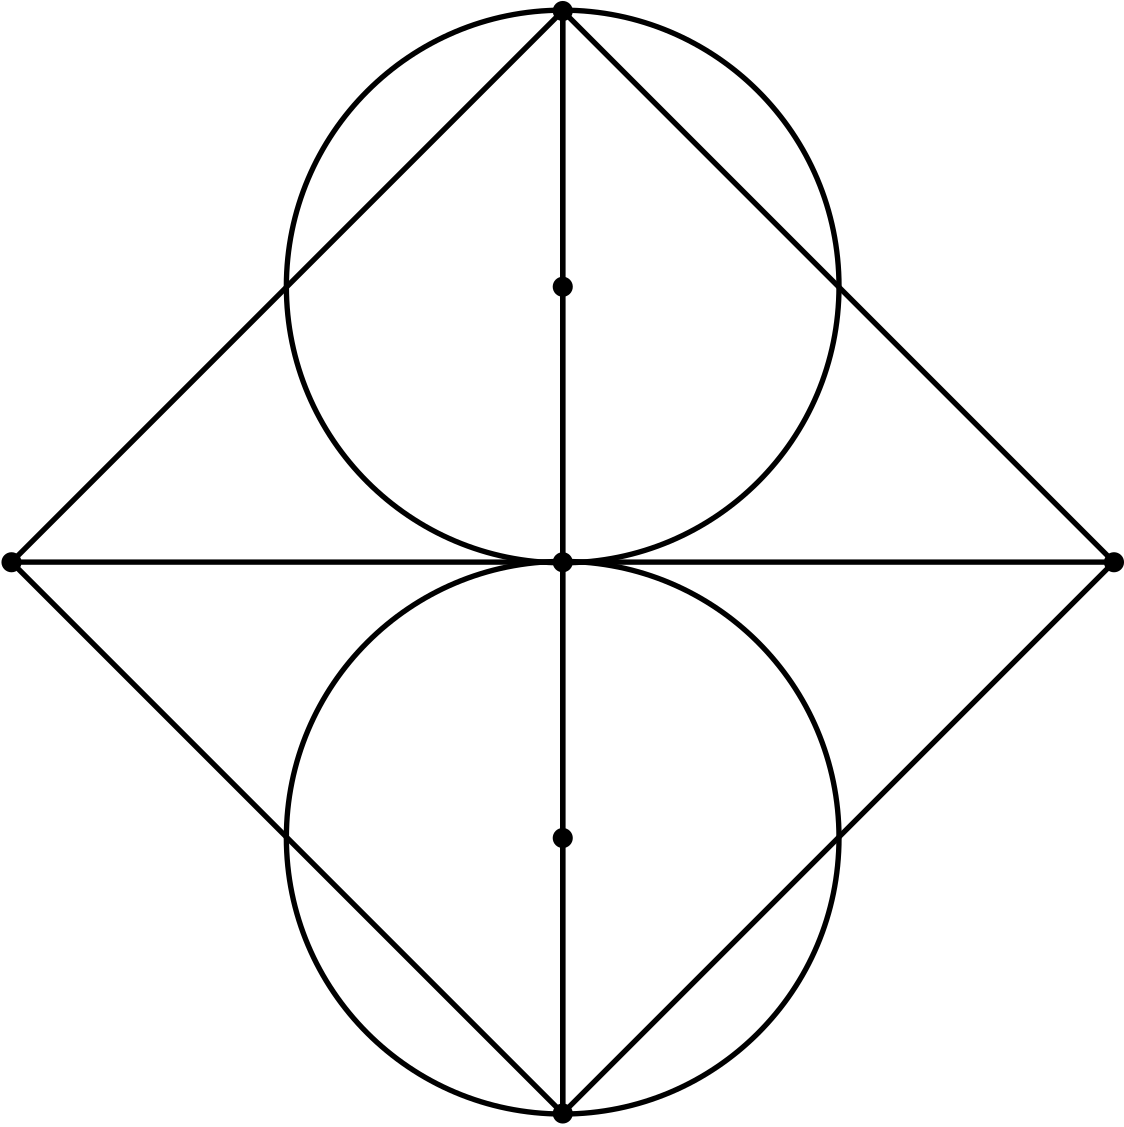
\includegraphics[height=12cm]{img/fig07.png}
\end{center}
\end{document}